\documentclass{article}
\usepackage{graphicx}
\usepackage[margin=1.5cm]{geometry}
\usepackage{csquotes}

\begin{document}

\title{Thursday Reading Assessment: Chapters 27-29 of \textit{Last Place on Earth}, Chapter 2 of \textit{Deep Survival}}
\author{Prof. Jordan C. Hanson}

\maketitle

\section{Memory Bank}

\begin{itemize}
\item One nautical mile corresponds to 1/60th of one degree, or 1.852 kilometers.
\end{itemize}

\section{Chapter 27 - Scott's Caravan}

\begin{enumerate}
\item Both Roal Amundsen and Robert Falcon Scott's strategies for moving gear and food South relied upon new motor sledge and diesel ship engine technologies.  Describe how each example helped the leaders achieve their goal.  What was the outcome of each effort? \\ \vspace{2cm}
\item Robert Falcon Scott used up to \textit{four} different kinds of transport as they began their journey.  The motor sledge was mentioned above.  What were the other three, and how did they compare in speed, and the ability to haul things? \\ \vspace{2cm}
\end{enumerate}

\section{Chapter 28 - The Devil's Ballroom}

\begin{enumerate}
\item \textbf{Amundsen chose as his average speed one degree of latitude every four days.} From page 412: ``Amundsen measured, indeed chose, his distances in degrees, not miles, so that effort was instinctively visualized on the surface of the globe, and thus the progress towards the goal, one of many little devices to keep up the spirits of the party.''  (Below in a footnote): ``An intelligent use of the powers of numbers and the significance of units.  The geographical, or nautical mile is one minute of latitude, or one sixtieth of a degree.  Nonetheless, the relation only makes an impact when simple fractions are involved.''  (a) How many kilometers is one degree of latitude?  (b) If Amundsen proceeded at this speed (one degree in four days), what was his speed in kilometers per hour?  \textit{Hint: convert the four days to hours for the time.} \\ \vspace{2cm}
\clearpage
\item When Amundsen's party reached the rolling hills at the edge of the interior of the Ross Ice shelf, they faced the prospect of climbing 14,000 ft up the central Trans-Antarctic mountains to get to the polar plateau.  Describe how they chose their pathway upwards and what they saw.  What was the effect on the men having such long visibility? \\ \vspace{2cm}
\begin{figure}
\centering
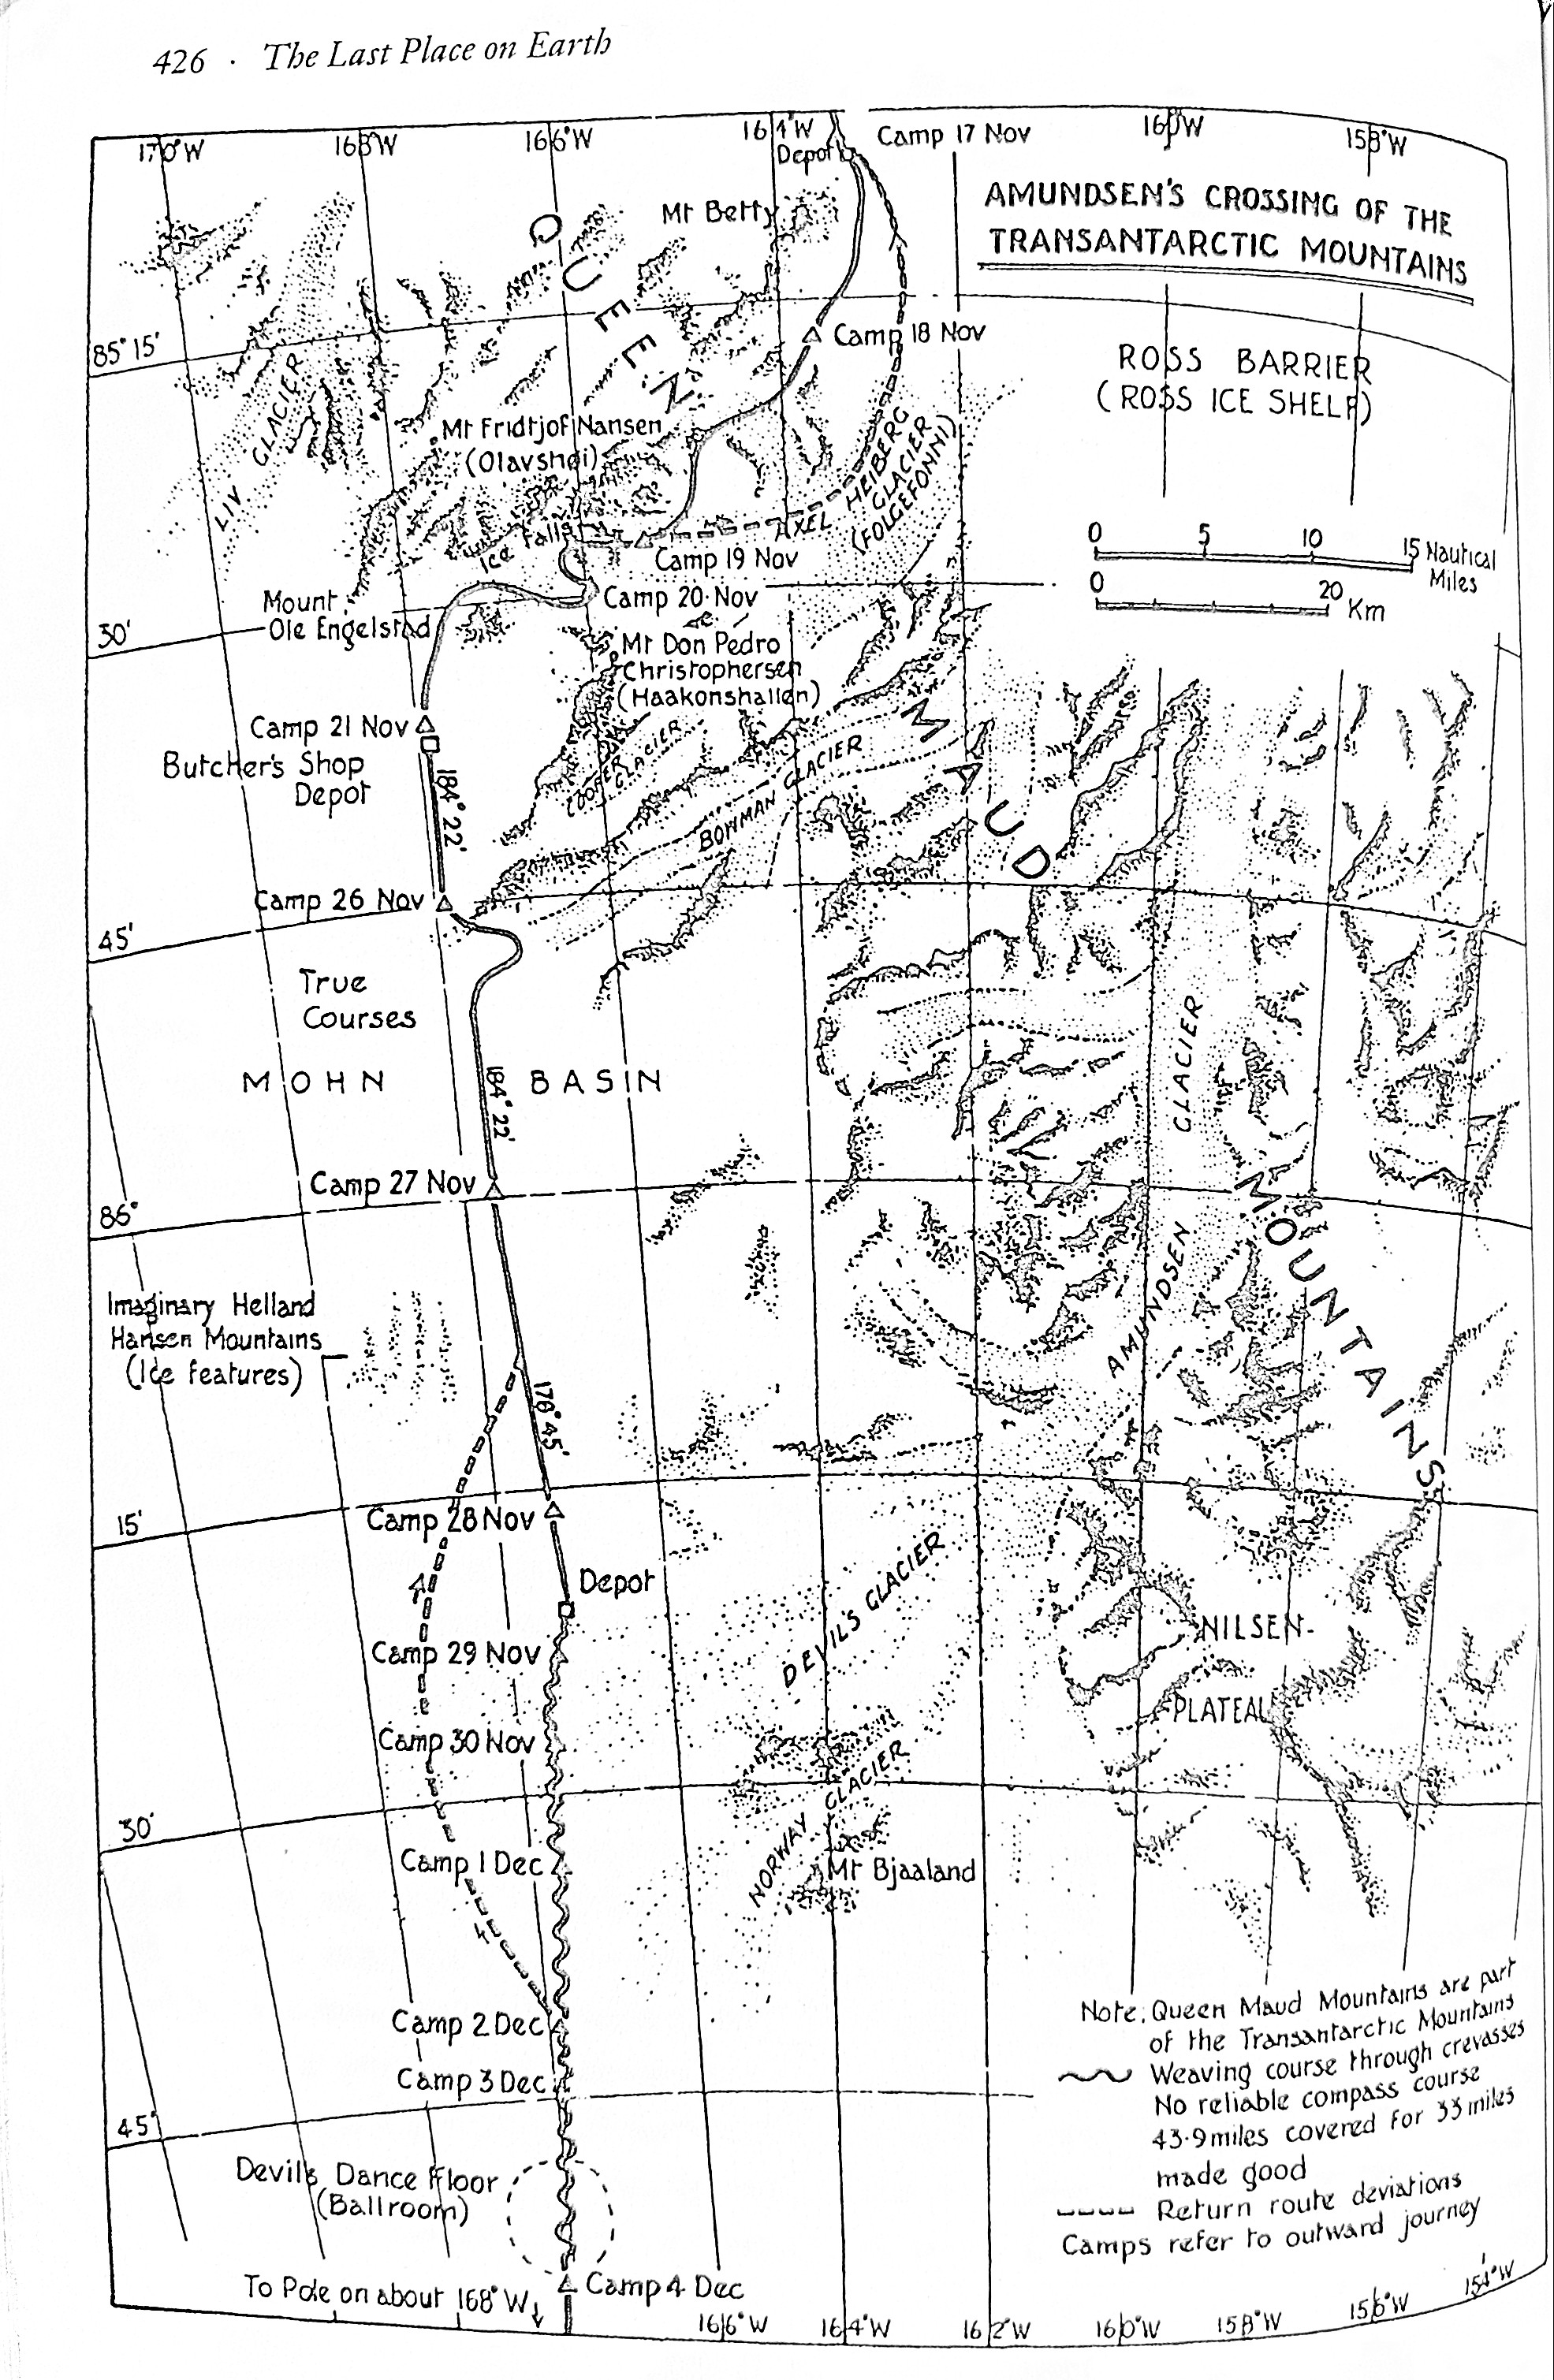
\includegraphics[width=0.4\textwidth]{map.jpg}
\caption{\label{fig:map} Amundsen's party moves through the central transantarctic mountains.}
\end{figure}
\end{enumerate}

\section{Chapter 29 - Man-Hauling Begins}
\begin{enumerate}
\item As the party of Scott reached the mountains they relieved themselves of the animals and began to pull the gear on their own.  Describe some of the technical deficiencies they experienced in their 10 miles per day. \\ \vspace{1cm} 
\end{enumerate}

\section{Chapter 2 of Deep Survival}

\begin{enumerate}
\item Do you recall how the snowmobile drivers wound up in an avalance?  Briefly, what was the answer to the author's rhetorical question: \textit{What were they thinking?}
\end{enumerate}

\end{document}
